\documentclass[11pt,a4paper]{article}
\author{TalentSprint}
\date{}
\usepackage{fancyhdr}
\usepackage{latexsym}
\usepackage{soul}
\usepackage{verbatim}
\usepackage{graphicx}
\usepackage{array}
\usepackage{enumerate}
%\usepackage{enumitem}
\usepackage{xcolor}
\usepackage[tikz]{bclogo}
\usepackage{textcomp}
\usepackage{latexsym}
\usepackage{seqsplit} 
\usepackage{setspace}
\usepackage{listings}
\lstset{language=html,numbers=left,numberstyle=\tiny,numbersep=10pt,showstringspaces=false}
\usepackage{fancyhdr}
\headheight=14pt
\lhead{\nouppercase{}}
\rhead{\nouppercase{\leftmark}}

\graphicspath{{../Images/}}

%\pagestyle{fancy}

%========================================================================

% Lengths and widths
\addtolength{\textwidth}{2.5cm}
\addtolength{\hoffset}{0cm}
\setlength{\headsep}{-12pt} % Reduce space between header and content
\setlength{\headheight}{85pt} % If less, LaTeX automatically increases it
\renewcommand{\footrulewidth}{2pt} % Remove footer line
\renewcommand{\headrulewidth}{1pt} % Remove header line
\renewcommand{\seqinsert}{\ifmmode\allowbreak\else\-\fi} % Hyphens in seqsplit
% This two commands together give roughly
% the right line height in the tables
\renewcommand{\arraystretch}{1.3}
\onehalfspacing



% Commands
\newcommand{\SetRowColor}[1]{\noalign{\gdef\RowColorName{#1}}\rowcolor{\RowColorName}} % Shortcut for row colour
\newcommand{\mymulticolumn}[3]{\multicolumn{#1}{>{\columncolor{white}}#2}{#3}} % For coloured multi-cols
\newcolumntype{x}[1]{>{\raggedright}p{#1}} % New column types for ragged-right paragraph columns
\newcommand{\tn}{\tabularnewline} % Required as custom column type in use

% Font and Colours
\definecolor{HeadBackground}{HTML}{333333}
\definecolor{FootBackground}{HTML}{666666}
\definecolor{TextColor}{HTML}{333333}
\definecolor{DarkBackground}{HTML}{6B8E23} %{FD1AA8}
\definecolor{LightBackground}{HTML}{E8FED8} %D3FDC8
\definecolor{tit}{HTML}{FF6600}
\renewcommand{\familydefault}{\sfdefault}
\color{TextColor}
 \headsep = 25pt
% Header and Footer
\pagestyle{fancy}
\usepackage[headheight=110pt]{geometry}
\fancyhf{}% Clear header/footer

\fancyhead[r]{
\includegraphics[width = 4cm, height = 2cm]{TS-Logo.png}\hspace{0cm}}

%=================================TITLE=====================================
\fancyhead[l]{\Large{\bf{\textcolor{tit}{\textrm{HTML - Frames and Forms}}}}}
%===========================================================================

\renewcommand{\headrulewidth}{0.4pt}% Default \headrulewidth is 0.4pt
\renewcommand{\footrulewidth}{0.4pt}% Default \footrulewidth is 0pt

\rfoot{Page \thepage}
\lfoot{COPYRIGHT \textcopyright TALENTSPRINT, 2015. ALL RIGHTS RESERVED.}




\begin{document}
\chapter*{Session 3 - Forms and frames} 
HTML forms provide a simple and reliable user interface to collect data from the user and transmit the data to a servlet or other server-side program for processing.

A form will take input from the site visitor and then will post your back-end application such as CGI, ASP Script or PHP script etc. Then your back-end application will do required processing on that data.

Elements like text fields, textarea fields, drop-down menus, radio buttons, checkboxes, etc. which are used to take information from the user.
\subsection*{How HTML Forms Transmit Data}
HTML forms let you create a variety of user interface controls to collect input in a Web page. Each of the controls typically has a name and a value, where the name is specified in the HTML and the value comes either from user input or from a default value in the HTML. The entire form is associated with the URL of a program that will process the data, and when the user submits the form (usually by pressing a button), the names and values of the controls are sent to the designated URL as a string of the form .

This string can be sent to the designated program in one of two ways: GET or POST. The first method, an HTTP GET request, appends the form data to the end of the specified URL after a question mark. The second method, HTTP POST, sends the data after the HTTP request headers and a blank line.

A simple syntax of using $<form>$ is as follows:
\begin{verbatim}
    <form action = "back-end script" method = "posting method">
        form elements like input, textarea etc.
    </form>
\end{verbatim}

Most frequently used form attributes are:
\begin{itemize}
\item \textbf{name:} This is the name of the form.
\item \textbf{action:} Here you will specify any script URL which will receive uploaded data.
\item \textbf{method:} Here you will specify method to be used to upload data. It can take various values but most frequently used are GET and POST.
\item \textbf{target:} It specifies the target page where the result of the script will be displayed. It takes values like \_blank, \_self, \_parent etc.
\end{itemize}

There are different types of form controls that you can use to collect data:
\begin{itemize}
\item Text input controls
\item Buttons
\item Checkboxes and radio buttons
\item Select boxes
\item File select boxes
\item Hidden controls
\item Submit and reset button
\end{itemize}

\subsection*{Text input controls}
HTML supports three types of text-input elements: textfields, password fields, and text areas. Each is given a name, and the value is taken from the content of the control.
The name and value are sent to the server when the form is submitted, which is typically done by means of a submit button.\\

There are actually three types of text input used on forms:
\begin{itemize}
\item \textbf{Single-line text input controls:} Used for items that require only one line of user input, such as search boxes or names. They are created using the $<input>$ element.
\item \textbf{Password input controls:} Single-line text input that mask the characters a user enters.
\item \textbf{Multi-line text input controls:} Used when the user is required to give details that may be longer than a single sentence. Multi-line input controls are created with the $<textarea>$ element.
\end{itemize}

Following is the list of attributes for $<input>$ tag.
\begin{itemize}
\item \textbf{type:} Indicates the type of input control you want to create. This element is also used to create other form controls such as radio buttons and checkboxes.
\item \textbf{name:} Used to give the name part of the name/value pair that is sent to the server, representing each form control and the value the user entered.
\item \textbf{value:} Provides an initial value for the text input control that the user will see when the form loads.
\item \textbf{size:} Allows you to specify the width of the text-input control in terms of characters.
\item \textbf{maxlength:} Allows you to specify the maximum number of characters a user can enter into the text box.
\end{itemize}

\subsubsection*{Single-line text input controls}
Single-line text input controls are created using an $<input>$ element whose type attribute has a value of text.\

\underline{\textbf{Example:}}
\begin{verbatim}
    <form>
        First name: 
            <input type = "text" name = "first_name" value = "Talent"/> <br>
        Last name: 
            <input type = "text" name = "last_name" value = "Sprint"/> <br>
            <input type = "submit" value = "submit" />
    </form>
\end{verbatim}
\textbf{Output:}\\
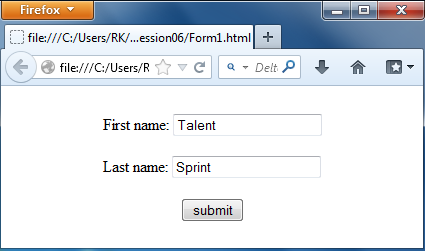
\includegraphics[height = 58mm, width = 120mm]{Form1.png}

\subsubsection*{Password input controls}
This is also a form of single-line text input controls are created using an $<input>$ element whose type attribute has a value of password.\\

\underline{\textbf{Example:}}
\begin{verbatim}
    <form>
        Login : 
        <input type = "text" name = "login" value = "Talent"/> <br>
        Password: 
        <input type = "password" name = "password" value = "Sprint"/> <br>
        <input type = "submit" value = "submit" />
    </form>
\end{verbatim}
\textbf{Output:}\\
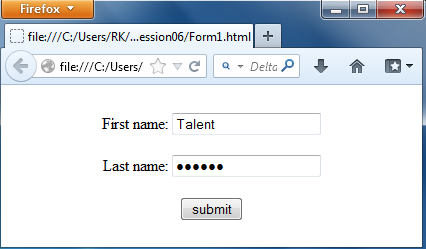
\includegraphics[height = 60mm, width = 120mm]{Form2.png}

\subsubsection*{Multiple-Line Text Input Controls}
If you want to allow a visitor to your site to enter more than one line of text, you should create a multiple-line text input control using the $<textarea>$ element.
\begin{verbatim}
    <form>
        Description : <br />
            <textarea rows = "5" cols = "50" name = "description">
                 Enter description here...
            </textarea>
            <input type = "submit" value = "submit" />
    </form>
\end{verbatim}
\textbf{Output:}\\
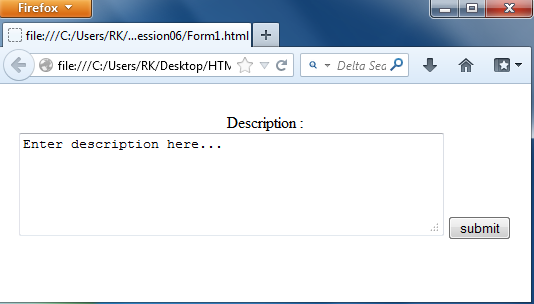
\includegraphics[height = 60mm, width = 110mm]{Form3.png}

Following is the detail of above used attributes for $<textarea>$ tag.
\begin{itemize}
\item \textbf{name:} The name of the control. This is used in the name/value pair that is sent to the server.
\item \textbf{rows:} Indicates the number of rows of text area box.
\item \textbf{cols:} Indicates the number of columns of text area box.
\end{itemize}
\subsection*{Creating Button}
The buttons are used for two main purposes in HTML forms, to submit forms and to reset the controls to the values specified in the original HTML. Browsers that use JavaScript can also use buttons for a third purpose, to trigger arbitrary JavaScript code.

Traditionally, buttons have been created by the INPUT element used with a TYPE attribute of SUBMIT, RESET, or BUTTON.

When you use the $<input>$ element to create a button, the type of button you create is specified using the type attribute.

The type attribute can take the following values:
\begin{itemize}
\item \textbf{submit:} This creates a button that automatically submits a form.
\item \textbf{reset:} This creates a button that automatically resets form controls to their initial values.
\item \textbf{button:} This creates a button that is used to trigger a client-side script when the user clicks that button.
\end{itemize}


\underline{\textbf{Example:}}\\
\begin{verbatim}
    <form>
        <input type = "submit" name = "Submit" value = "Submit" />
        <br /><br />
        <input type = "reset" value = "Reset" />
        <input type = "button" value = "Button"  />
    </form>
\end{verbatim}

\textbf{Output:}\\
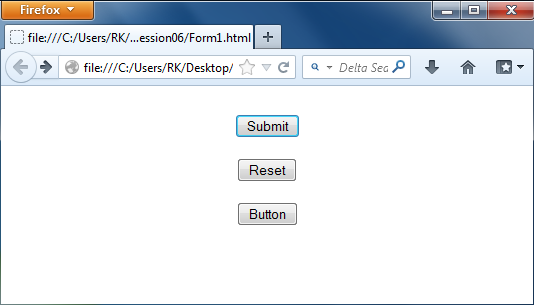
\includegraphics[height = 60mm, width = 100mm]{Form4.png}\\

\underline{\textbf{Example:}} \textbf{Using an image to create a button.}\\
\begin{verbatim}
    <form >
        <input type = "image" name = "imagebutton" src = "URL" />
    </form>
\end{verbatim}

\textbf{Output:}\\
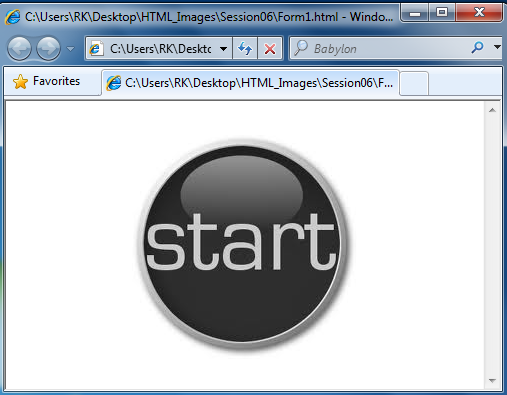
\includegraphics[height = 60mm, width = 100mm]{Form5.png}

\emph{Note:Here src attribiute specifies a location of the image on your webserver.}\\

\underline{\textbf{Example:}} Using $<button>$ element to create various buttons\\
\begin{verbatim}
    <form>
        <button type = "submit">Submit</button>
        <br /><br />
        <button type = "reset"> Reset </button>
        <button type = "button"> Button </button>
    </form>
\end{verbatim}

\textbf{Output:}\\

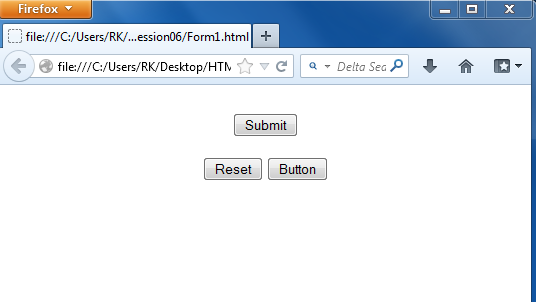
\includegraphics[height = 60mm, width = 110mm]{Form6.png}\\

\subsection*{Checkboxes Control}
Checkbox buttons allows the user to select one or more options among a set of predefined choices. They are created using $<input>$ tag.

Following is the list of important checkbox attributes:

\begin{itemize}
\item \textbf{type:} Indicates that you want to create a checkbox.
\item \textbf{name:} Name of the control.
\item \textbf{value:} The value that will be used if the checkbox is selected. More than one checkbox should share the same name only if you want to allow users to select several items from the same list.
\item \textbf{checked}: Indicates that when the page loads, the checkbox should be selected.
\end{itemize}
\underline{\textbf{Example:}}
\begin{verbatim}
    <form>
        <input type = "checkbox" name = "SSS" value = "on"> SSC
        <input type = "checkbox" name = "Inter" value = "on"> INTER
        <input type = "checkbox" name = "Graduation" value = "on"> Graduation
        <input type = "submit" value = "Select" />
    </form>
\end{verbatim}
\underline{\textbf{Output:}}\\
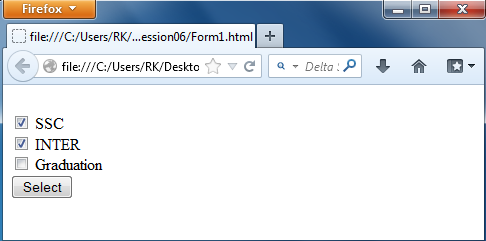
\includegraphics[height = 60mm, width = 110mm]{Form7.png}
\subsection*{Raido box Control}
Radio Buttons are used when only one option is required to be selected. radio buttons can be grouped so that only a single member of the group can be selected at a time.

Radio buttons differ from check boxes in that only a single radio button in a given group can be selected at any one time. You indicate a group of radio buttons by providing all of them with the same NAME. Only one button in a group can be depressed at a time, selecting a new button when one is already selected results in the previous choice becoming deselected. The value of the one selected is sent when the form is submitted.\\

Following is the list of important radiobox attributes:
\begin{itemize}
\item \textbf{type:} Indicates that you want to create a radiobox.
\item \textbf{name:} Name of the control.
\item \textbf{value:} Used to indicate the value that will be sent to the server if this option is selected.
\item \textbf{checked:} Indicates that this option should be selected by default when the page loads.
\end{itemize}
\underline{\textbf{Example:}}
\begin{verbatim}
    <form>
        <input type = "radio" name = "Qualification" value = "SSC"> SSC
        <input type = "radio" name = "Qualification" value = "Inter"> INTER
        <input type = "radio" name = "Qualification" value = "Graduation"> 
                                                       Graduation
        <input type = "submit" value = "Select" />
    </form>
\end{verbatim}
\underline{\textbf{Output:}}\\
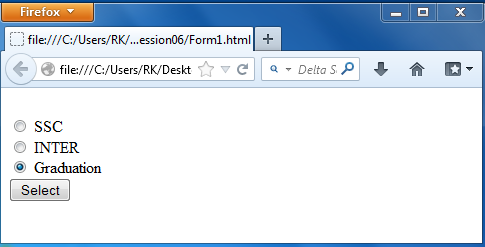
\includegraphics[height = 53mm, width = 120mm]{Form8.png}
\subsection*{Select box Control}
A SELECT element presents a set of options to the user. You specify each choice with an OPTION element enclosed between$<SELECT ...>$ and $</SELECT ...>$.

Following is the list of important attributes of $<select>$:
\begin{itemize}
\item \textbf{name:} This is the name for the control.
\item \textbf{size:}This can be used to present a scrolling list box.
\item \textbf{multiple:} If set to "multiple" then allows a user to select multiple items from the menu.
\end{itemize}

Following is the list of important attributes of $<option>$:
\begin{itemize}
\item \textbf{value:} The value that is sent to the server if this option is selected.
\item \textbf{selected:} Specifies that this option should be the initially selected value when the page loads.
\item \textbf{label:} An alternative way of labeling options.
\end{itemize}
\underline{\textbf{Example:}} of a SELECT menu\\
\begin{verbatim}
    <SELECT NAME = "language">
        <OPTION VALUE = "c">C
        <OPTION VALUE = "c++">C++
        <OPTION VALUE = "java" SELECTED>Java
        <OPTION VALUE = "lisp">Lisp
        <OPTION VALUE = "perl">Perl
        <OPTION VALUE = "smalltalk">Smalltalk
    </SELECT>
\end{verbatim}
\textbf{Output:}\\
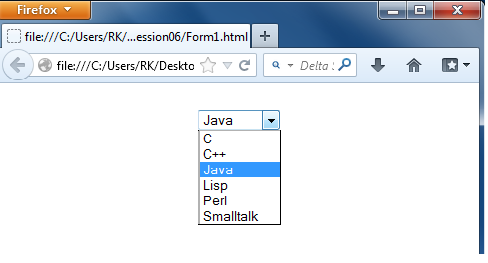
\includegraphics[height = 60mm, width = 110mm]{Form9.png}

\underline{\textbf{Example:}} of a SELECT menu that permits selection of multiple options\\
\begin{verbatim}
    Languages you know:<BR>
    <SELECT NAME = "language" MULTIPLE>
        <OPTION VALUE = "c">C
        <OPTION VALUE = "c++">C++
        <OPTION VALUE = "java" SELECTED>Java
        <OPTION VALUE = "lisp">Lisp
        <OPTION VALUE = "perl" SELECTED>Perl
        <OPTION VALUE = "smalltalk">Smalltalk
    </SELECT>
\end{verbatim}


\underline{\textbf{Output:}}

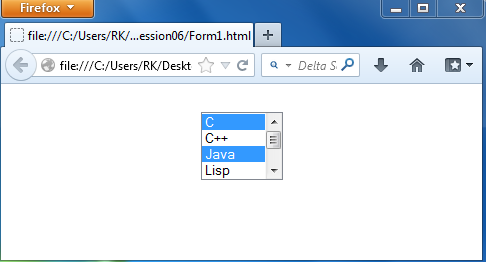
\includegraphics[height = 75mm, width = 120mm]{Form10.png}

\underline{\textbf{Example:}} SELECT menu categorized into two groups with the OPTGROUP element
\begin{verbatim}
    Server-side Languages:
    <SELECT NAME = "language">
        <OPTGROUP LABEL = "Common Servlet Languages">
            <OPTION VALUE = "java1">Java
        </OPTGROUP>
        <OPTGROUP LABEL = "Common CGI Languages">
            <OPTION VALUE = "c">C
            <OPTION VALUE = "c++">C++
            <OPTION VALUE = "java2">Java
            <OPTION VALUE = "perl">Perl
            <OPTION VALUE = "vb">Visual Basic
        </OPTGROUP>
    </SELECT>
\end{verbatim}
\underline{\textbf{Output:}}

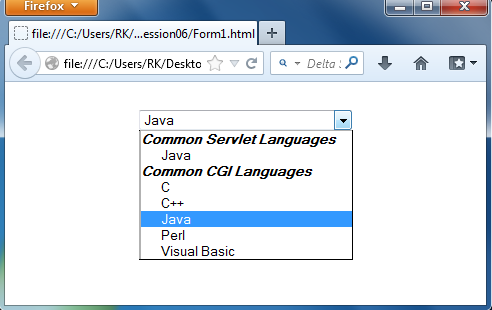
\includegraphics[height = 60mm, width = 110mm]{Form11.png}
\subsection*{Hidden Controls}
If you will want to pass information between pages without the user seeing it. Hidden form controls remain part of any form, but the user cannot see them in the Web browser. They should not be used for any sensitive information you do not want the user to see because the user could see this data if she looked in the source of the page.\\

\underline{\textbf{Example:}}
\begin{verbatim}
    <form method = "get" name = "pages">
        <p>This is page 10</p>
        <input type = "hidden" name = "pagenumber" value = "10" />
        <input type = "submit" value = "Next Page" />
    </form>
\end{verbatim}
\underline{\textbf{Output:}}

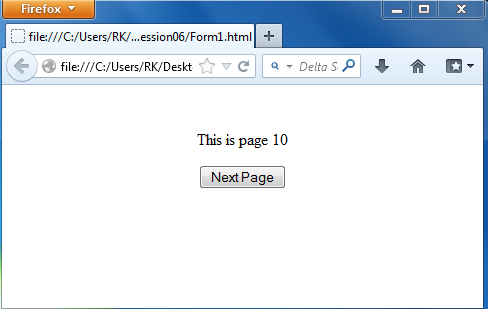
\includegraphics[height = 52mm, width = 120mm]{Form12.png}

\subsection*{HTML5 New Input Types}
HTML5 has several new input types for forms. These new features allow better input control and validation.

\begin{tabular}{|l|l|}\hline
\multicolumn{1}{ |c| }{\textbf{Tag}} & \multicolumn{1}{ |c| }{\textbf{Description}} \\ \hline

$<datalist>$ & 	Specifies a list of pre-defined options for an $<input>$  element\\ \hline
$<keygen>$ & 	Specifies a key-pair generator field in a form\\ \hline
$<output>$ &	Represents the result of a calculation\\ \hline

$<color>$ & Used for input fields that should contain a color.\\ \hline
$<date>$ & Allows the user to select a date.\\ \hline
$<datetime>$ & Allows the user to select a date and time (with time zone).\\ \hline
$<datetime-local>$ & Allows the user to select a date and time (no time zone).\\ \hline
    $<email>$ & Defines an input fields that should contain an e-mail address.\\ \hline
    $<month>$ & Allows the user to select a month and year.\\ \hline
    $<number>$ & Defines an input fields that should contain a numeric value.\\ \hline
    $<range>$ & Defines an input fields that should contain a value \\ & from a range of numbers.\\ \hline
    $<search>$ & Used for search fields\\ & (a search field behaves like a regular text field).\\ \hline
    $<tel>$ & Defines an input fields that should contain a telephone number. \\ \hline
    $<time>$ & Defines a control for entering a time (no time zone)\\ \hline
    $<url>$ & Defines a field for entering a URL\\ \hline
    $<week>$ & Defines a week and year control (no time zone)\\ \hline
\end{tabular}
 
\subsection*{HTML5 New Attributes}
HTML5 has provided new attributes for $<form>$ and $<input>$.

\subsection*{New $<form>$ Attributes}
\begin{description}
\item [autocomplete] - The autocomplete attribute specifies whether a form or input field should have autocomplete-on or off. When autocomplete is on, the browser automatically complete values based on values that the user has entered before.
\emph{Note: The autocomplete attribute works with $<form>$ and the following $<input>$ types: text, search, url, tel, email, password, datepickers, range, and color.}

\item[novalidate] -The novalidate attribute is a boolean attribute. When present, it specifies that the form-data (input) should not be validated when submitted.
\end{description}

\subsubsection*{New $<input>$ Attributes}
\begin{description}
\item [autofocus] - The autofocus attribute is a boolean attribute. When present, it specifies that an $<input>$ element should automatically get focus when the page loads.
\item [form] - The form attribute specifies one or more forms an $<input>$ element  belongs to.
\item [formmethod] - The formmethod attribute overrides the method attribute of the $<form>$ element.
\item [min and max] - The min and max attributes specify the minimum and maximum value for an $<input>$ element.
\item [placeholder] - The placeholder attribute specifies a short hint that describes the expected value of an input field (e.g. a sample value or a short description of the expected format).
\item [required] - It specifies that an input field must be filled out before submitting the form.
\end{description}

\subsubsection*{Examples}
\begin{description}
\item [Exampe-01]

Sample code to play Video Clip

\begin{lstlisting}
<DOCTYPE html>
    <html>
        <head>
            <title> HTML5 Video </title>
        </head>
        <body>
            <center>
                <video width="320" height="240" controls>
                    <source src="./media/movie1.mp4" 
                                        type="video/mp4">
                    <source src="./media/movie1.ogg" 
                                       type="video/ogg">
                    Your browser does not support the video tag.
                </video> 
                <h1> <u>This is a video player.</u></h1>


            </center>
        </body>
    </html>
\end{lstlisting}

\item [Example-02]

Sample code to play Audio Clip

\begin{lstlisting}
<DOCTYPE html>
    <html>
        <head>
            <title> HTML5 Audio</title>
        </head>
        <body>
            <center>
                
                <audio controls>
                    <source src="./media/audio1.ogg" 
                                           type="audio/ogg">
                    <source src="./media/audio1.mp3" 
                                           type="audio/mpeg">
                    Your browser does not support the audio element.
                </audio>
		<h1> <u>This is an audio player.</u></h1>

            </center>
        </body>
    </html>
\end{lstlisting}
\end{description}

%====================================================================================================================================
%====================================================================================================================================

\subsection*{New Elements in HTML5}
\subsubsection*{What’s new?}
\hspace{20pt}HTML5 was created to make the coding process easier and more logical. The unique and impressive features HTML5 comes with are in the multimedia department. Many of the features it comes with have been created with the consideration that users should be able to run heavy content on low-powered devices. The syntactic features include the new $<video>$, $<audio>$ and $<canvas>$ elements, but also integration of vector graphics content (what we knew before as being the $<object>$ tags). This means that multimedia and graphic content on the web will be handled and executed easier and faster, without the need of plugins or APIs.

\subsubsection*{New Elements}

\begin{tabular}{|l|l|}\hline
\multicolumn{1}{ |c| }{\textbf{Tag}} & \multicolumn{1}{ |c| }{\textbf{Description}} \\ \hline
$<article>$  &	Defines an article in the document \\ \hline
$<aside>$ &	Defines content aside from the page content \\ \hline
$<audio>$ &     Defines sound, such as music or other audio streams.\\ \hline
$<video>$ &    Defines video, such as a movie clip or other video streams.\\ \hline
$<source>$ &    is used to specify multiple media resources for media elements,\\ & such as $<video>$ and $<audio>.$ \\ \hline
$<bdi>$ &	Defines a part of text that might be formatted in a \\ & different direction from other text outside it \\ \hline
$<details>$ & 	Defines additional details that the user can view or hide \\ \hline
$<dialog>$  & 	Defines a dialog box or window\\ \hline
$<figcaption> $  &	Defines a caption for a $<figure>$ element \\ \hline
$<figure>$  &	Defines self-contained content, like illustrations,\\ & diagrams, photos, code listings, etc. \\ \hline
\end{tabular}

\pagebreak

\begin{tabular}{|l|l|}\hline
\multicolumn{1}{ |c| }{\textbf{Tag}} & \multicolumn{1}{ |c| }{\textbf{Description}} \\ \hline
$<footer>$  & 	Defines a footer for the document or a section \\ \hline
$<header>$  & 	Defines a header for the document or a section \\ \hline
$<main>$  & 	Defines the main content of a document \\ \hline
$<mark>$  & 	Defines marked or highlighted text \\ \hline
$<menuitem>$  &  	Defines a command/menu item that the user can\\ & invoke from a popup menu \\ \hline
$<meter>$  & 	Defines a scalar measurement within a known range\\ \hline
$<nav>$  & 	Defines navigation links in the document \\ \hline
$<progress>$  &	Defines the progress of a task \\ \hline
$<rp>$  &	Defines what to show in browsers that do not support\\ & ruby annotations \\ \hline
$<rt>$  & 	Defines an explanation/pronunciation of characters \\ &(for East Asian typography) \\ \hline
$<ruby>$  &	Defines a ruby annotation (for East Asian typography) \\ \hline
$<section>$  & 	Defines a section in the document \\ \hline
$<summary>$  & 	Defines a visible heading for a $<details>$ element \\ \hline
$<time>$  &	Defines a date/time \\ \hline
$<wbr>$  & 	Defines a possible line-break \\ \hline
\end{tabular}

\end{document}
